As a complementary approach to the input output method, we use the dynamic macroeconomic cge-model GreenREFORM, currently under development by DREAM-gruppen (see \cite{GR_status} for latest project status), to calculate price and wage changes after a carbon tax. This approach will able us to analyze how big an impact general equilibrium effects have for the results. The GreenREFORM model is calibrated to the emission projections of the \cite{kf21}, thus the emissions are compatible with the input output analysis.

\subsection{Calculating price changes} In this section we explain how we calculate the prices and wage to be inserted in our partial demand model.

The Green Reform model is based on the 117 sectors from the national accounting of Statistics Denmark, where the agricultural sector, transport sector and renovation sector are further divided into detailed sectors that have different environmental impacts \citep{GR_brancher}. For instance the agricultural sector is divided into meat and plant production, transport into electrical end gas vehicles (see a list of all the 53 sectors in the table below). Other sectors (mainly service) are aggregated due to their low  environmental impact. 
Further the sector good-based accounting is accompanied by an energy accounting consisting of 43 different energy goods (coal, oil, petroleum, electricity, wood, etc.). The energy goods are grouped by their purpose (transport, heating, process, etc.), since energy taxes differ by energy purpose. 
When calculating CO2e-emissions in the model, emissions from the sector's output are entirely non-energy related, while all the energy related emissions stem from the energy goods.
\\
\\
Running experiments with the GreenREFORM model, we get a consumer price index for each sector's output (including consumption taxes) and for each energy good, before and after a carbon tax. The price index is a CES-index between imported and domestically produced goods. The assumed elasticity of substitution between imported and domestic goods equals to 1.25 for all goods. Since there is no distinction between domestically produced and imported goods in the consumer-survey data, we find this the appropriate price index. Further, using this index we incorporate the effect of increased foreign competition due to a domestic tax increase in our results.

For our two energy consumption groups: Energy for housing and Energy for transport, we can use the energy prices directly from GreenREFORM. Since these two purposes match the GreenREFORM purposes, we can use the price index that is aggregated across energy goods. The price increase for these two consumption groups corresponds to the direct  carbon tax payments for households.

For the remaining consumption groups, we calculate the prices, by constructing a mapping from the GreenREFORM sectors to the available 69 sector aggregation of Statistics Denmark's NIO1 table from 2018. This requires an aggregation of both the GreenREFORM sectors and the NIO1-69 sectors. The result is 30 aggregated sectors shown in the table below. The NIO1 table is selected such that demand is divided into the 74 consumption groups of the National Accounting, which are then aggregated to our 8 consumption groups. We sum the purchase of domestically and imported consumption. Since the 74 consumption group division is clearly divided by meat and non-meat consumption, we can split the agricultural sector of the NIO69 into a meat and non-meat sector, to get the most accurate price increase for meat and dairy. 

 The price changes in each year is calculated as the price development after a carbon tax divided by the baseline price development, which equals 1 in t0: 
\begin{align}
    \Delta p_{s30,t} = \frac{p_{s30,t,tax}}{p_{s30,t,baseline}},
\end{align}

The price after a tax for each of the consumption groups (leaving out the energy groups) is then calculated as a Laspeyres price index across sectors:
\begin{align}
    p_{g,t} = \frac{\sum_{s30}(\Delta p_{s30,t}v_{s30,g,t0})}{\sum_{s30} (v_{g,s30,t0})}
\end{align}
where $g$ stands for the consumption groups: Meat and dairy, Other foods, Housing, Transport, Other goods and Other services, $s30$ stands for the 30 sectors in the aggregation and $t$ is the time from 2018 to 2040. $v_{s,g,t}$ is thus the value of output produced by sector $s30$ belonging to consumption group $g$. 

From the experiments we also extract the real wage rate before tax. The wage rate to be used in our partial demand model is calculated similar to the price changes, as: 
\begin{align}
    w_t =\frac{w_{t,tax}}{w_{t,baseline}},
\end{align}
and is used to calculate changes in total expenditure and disposable income. In the CGE model all prices are inflation adjusted, quantities are growth adjusted and values are both inflation and growth adjusted. The wage is treated like a value, since labor is a fixed factor in production \citep{GR_reform}, thus it is also growth adjusted. We only use the wage rate to calculate changes in income and total consumption. Thus, letting income and consumption grow in our demand system corresponds to letting the wage grow. The only minor difference, is that GreenREFORM has adjusted with an average growth rate of 1.5 percent, while our system grows with 1.44 percent.
%In the model labor is a fixed factor and there exist a structural unemployment fraction. When demand changes in the model, labor moves freely between sectors, until the model clears.


\subsection{Price and wage changes for three different tax scenarios}\label{sec:tax_pd}
We will consider three different tax scenarios, which are listed below. All three taxes are phased in linearly during 2026-2030. The taxes are announced in 2040, such that there exist anticipation effects.
\begin{itemize}
    \item The first scenario is a uniform CO2e tax of 1500 DKK as recommended by \cite{klimaraad2021} (er det korrekt). This implies that existing energy taxes will be phased out. 
    \item The second scenario is a CO2e tax of 1250 DKK on top of existing energy taxes. If politicians decide to keep the existing energy taxes, it is likely that the CO2e tax will be smaller, which is why we chose a lower tax rate.
    \item The third scenario is a uniform CO2e tax of 1500 DKK, where the Green REFORM model is changed to have an exogenous rental price on land. This is because when land is assumed to be a fixed factor the price on land drops heavily when demand is reduced, and this affects prices in the agricultural sectors.
\end{itemize}

 Running the three different scenarios give different price changes that evolve over time. Two snapshots are presented in table \ref{tabel_dp} for the year 2027, when the tax has just been implemented, and the year 2035, when prices are fairly constant again. Overall the tax three reforms yield similar results: The price of meat and dairy and other foods increases by less than a half percent in 2035. The price of housing drops by half percent. The price of energy for housing increases with 1.5-2 percent. The price of energy for transport increases heavily between 15 and 18 percent. The price of transport and other goods decreases with up to a half percent, and other services decreases with almost 1 percent. Finally the wage rate decreases around 2 percent. 
- refer to DØRS' poitive price effect.


\begin{table}[hhh]
\caption{Price and wage changes in 2027 and 2035 for 3 different tax scenarios}
\label{tabel_dp}
\begin{tabular}{@{}lllllll@{}}
\toprule
CO2e tax: & \multicolumn{2}{l}{\begin{tabular}[c]{@{}l@{}}1500 DKK  \\ Uniform   \end{tabular}} & \multicolumn{2}{l}{\begin{tabular}[c]{@{}l@{}}1250 DKK\\ On top of energy taxes\end{tabular}} & \multicolumn{2}{l}{\begin{tabular}[c]{@{}l@{}}1500 DKK\\ Uniform exo. land price\end{tabular}} \\ \midrule
\textbf{Year} & \textbf{2027} & \textbf{2035} & \textbf{2027} &\textbf{2035} & \textbf{2027} & \textbf{2035} \\
Meat and dairy & 0.998 & 1.004 \thickspace \thickspace \thickspace \thickspace \thickspace \thickspace \thickspace \thickspace \thickspace \thickspace \thickspace \thickspace  & 0.998 & 1.003 & 0.998 & 1.006 \\
Other foods & 0.998 & 1.003 & 0.998 & 1.002 & 0.998 & 1.005 \\
Housing & 0.987 & 0.995 & 0.988 & 0.995 & 0.986 & 0.994 \\
Energy, housing & 1.007 & 1.016 & 1.009 & 1.019 & 1.007 & 1.017 \\
Energy, transport & 1.064 & 1.150 & 1.077 & 1.180 & 1.064 & 1.150 \\
Transport & 0.996 & 0.999 & 0.997 & 0.999 & 0.995 & 0.998 \\
Other goods & 0.994 & 0.995 & 0.995 & 0.995 & 0.993 & 0.994 \\
Other services & 0.992 & 0.992 & 0.992 & 0.993 & 0.990 & 0.991 \\
Wage rate & 0.985 & 0.983 & 0.986 & 0.984 & 0.982 & 0.979 \\ \bottomrule
\end{tabular}
\caption*{
\textbf{Source:} Own calculations based on the GreenREFORM model}
\end{table}


Except for energy for housing and energy for transport, these price increases are way lower than what we get from using the input output method, see table \ref{pchange1250}. For especially Meat and Dairy and Other foods the price increases are below what one might expects given that agriculture, forestry and fishery stands for 26 percent of domestic emissions \citep[Table DRIVHUS]{statbank}. Further, the prices of the less CO2 intensive goods actually fall. This is all due to general equilibrium effects.
\\
\\
There are a lot of different mechanisms at play in the general equilibrium model. Here we will mention a few of them. First of all, the general equilibrium model will capture the effect that when prices increase, demand for products is reduced, which makes prices fall. Another important mechanism is that GreenREFORM models foreign competition. Since we analyze a domestic carbon tax, prices of foreign goods are kept constant. The prices consumers faces are indexes between domestic and foreign and domestic goods, thus the price increase of goods will be smaller than in a closed economy, as is considered in the input output analysis. Further, when domestic prices are increased, firms and households substitute towards foreign goods. To avoid losing large market shares, domestic firms are 'forced' to lower input prices in order to keep their product competitive.
An important consequence of the firms' need to ensure rentability compared to foreign firms, is that the wage rate is pushed downwards. Firms will substitute towards more labor as production-input, and since labor is fixed, output is reduced further \citep{Simpel_co2skat}.
\\
 
The prices for agricultural sectors are determined by the agricultural model of GreenREFORM \citep{GR_landbrug}. In this module land use is modeled as a production input of the vegetable sectors. It is assumed that the amount of land is fixed, due to a recognition that land taken out of production will quickly be utilized again, and that the price adjusts. Due to the endogenous modeling of the rental price, the CO2 tax leads to a decreased demand of land, that reduces the rental price of land by around 47 pct in 2030 for the two tax scenarios with endogenous price on land. In GreenREFORM land is owned by the vegetable producers, thus this effect is mainly of importance for these sectors. However, the lower rental price can carry over to the output prices of all the agricultural sectors, since the meat producing sectors buy among others manure from the vegetable sectors. The third tax scenario with an exogenous rental price on land is done to see how much the assumption of endogenous land price affects consumer prices when imposing a CO2e tax. As seen from table \ref{tabel_dp}, the price on meat and dairy and other foods do increase a bit more when removing this mechanism, but it seem that the wage rate is then further reduced to ensure firms' rentability, such that the overall price level is kept down.

\subsection{Distributional effects from a CO2e tax of only price changes}
In order to calculate the distributional effects of the tax reforms, we input the price and wage changes into our dynamic partial consumer model, as described in section \ref{sec:partialmodel}. We consider a case where total income and total expenditure across quintiles grows with the average growth rate of 1.44 percent per year, thus we incorporate LES income effects, as printed in table \ref{wtable}.
\\

Below we present the distributional effects of price changes measured as the $EV_P$ relative to total expenditure and disposable income. The $EV_p$ is calculated as described in section \ref{sec:measurewelfare}. The $EV_P$ is essentially a measure of the price of the quintiles' consumption bundles. That is a price index, which is weighted with the quantity of the different consumption groups. As can be seen in figure \ref{tax1_EVP} to figure \ref{tax3_EVP}, the distributional effect of increased prices is actually positive and progressive up to 2030, and thereafter it is slightly negative and slightly regressive. The largest negative and regressive outcome is seen in the case of a 1250 DKK carbon tax on top of energy taxes.

\begin{figure}[H]
\centering
\caption{EV$_P$ relative to total expenditure and disposable income from a uniform 1500 CO2e tax}
\label{tax1_EVP}
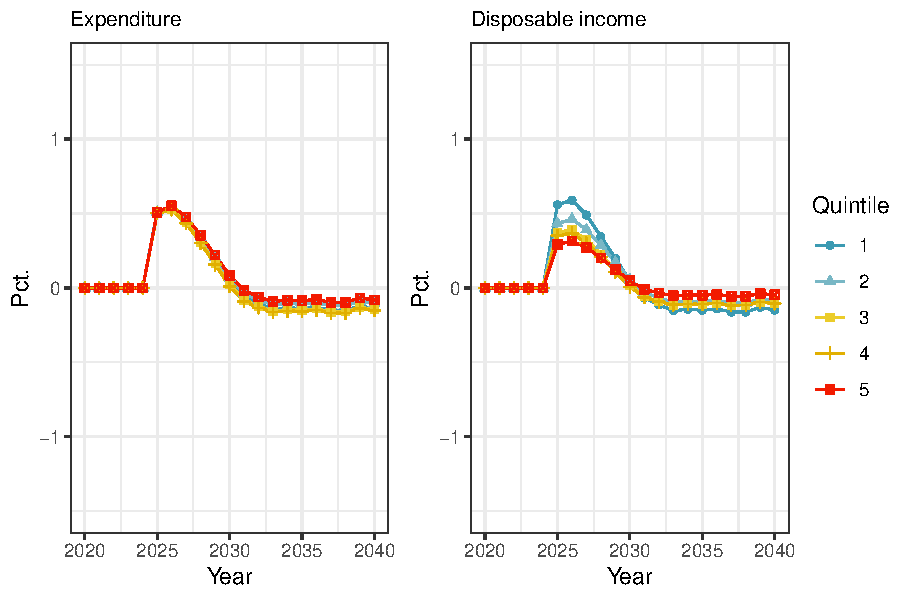
\includegraphics[width=.9\textwidth]{Figures/EV_P_tax1.pdf}
\captionsetup{singlelinecheck=off,size=scriptsize}
\setlength{\captionmargin}{10pt}
\caption*{
\textbf{Note:} ??\\
\textbf{Source:} Own calculations based on the GreenREFORM model}
\end{figure}


\begin{figure}[H]
\centering
\caption{EV$_P$ relative to total expenditure and disposable income from a 1250 CO2e tax on top of energy taxes}
\label{tax2_EVP}
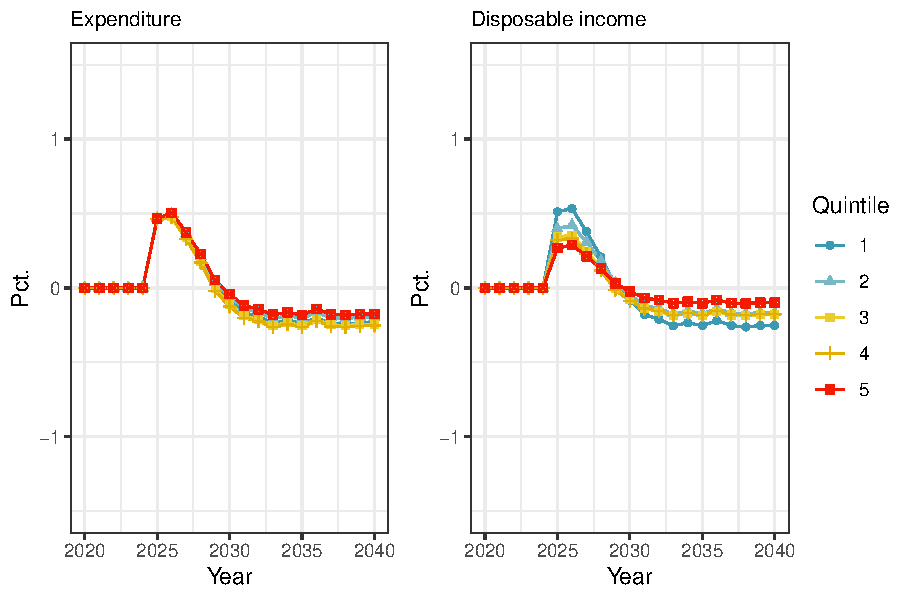
\includegraphics[width=.9\textwidth]{Figures/EV_P_tax2.pdf}
\captionsetup{singlelinecheck=off,size=scriptsize}
\setlength{\captionmargin}{10pt}
\caption*{
\textbf{Note:} ??\\
\textbf{Source:} Own calculations based on the GreenREFORM model}
\end{figure}


\begin{figure}[H]
\centering
\caption{EV$_P$ relative to total expenditure and disposable income from a uniform 1500 CO2e tax where land price is exogenous}
\label{tax3_EVP}
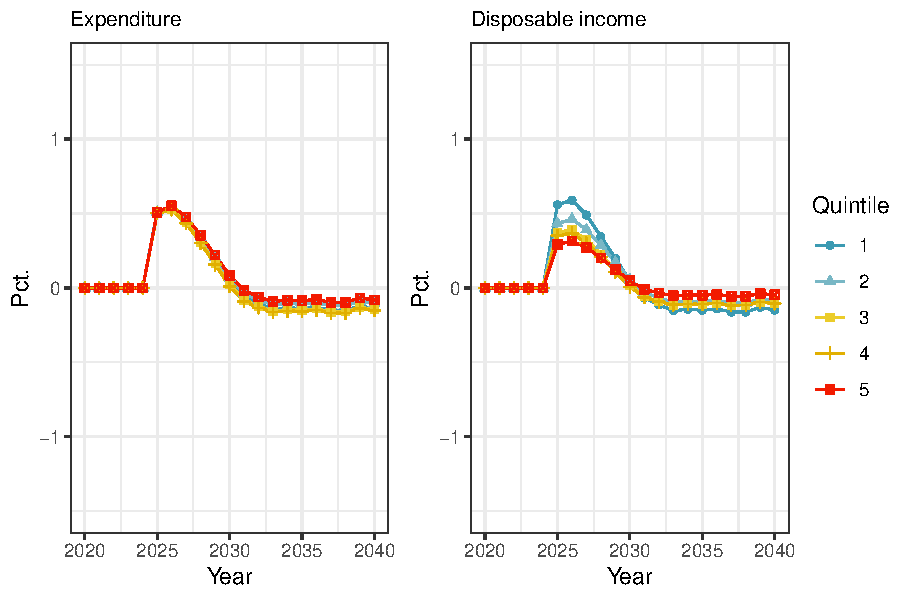
\includegraphics[width=.9\textwidth]{Figures/EV_P_tax1.pdf}
\captionsetup{singlelinecheck=off,size=scriptsize}
\setlength{\captionmargin}{10pt}
\caption*{
\textbf{Note:} ??\\
\textbf{Source:} Own calculations based on the GreenREFORM model}
\end{figure}


There are some opposite effects for the distributional outcome. Energy for housing, meat and dairy and other foods increases in price, which makes the outcome regressive, since it takes up a larger share on the lower quintiles' budget, as can be seen in table \ref{figshare}. On the other side, energy for transport is the consumption group that increases most heavily in price, and this group takes up the largest share of the higher quintiles' consumption bundle, making the outcome more progressive.

Further we see that other services make up between 20 and 25 percent of consumers' budget in 2019. The GreenREFORM sector: Financial service activities, except insurance and pension funding, which contains rental for non-residential housing, drops by 1.5 percent in 2030 and 1.3 percent in 2040. Looking closer into the input-output tables on which the model is built (\cite{statbank}, table NIO1), it is seen that every other sector takes large inputs from this sector in production, which contributes to the price decrease. Further this sector makes up 25 percent of the consumption group other services. The shift towards services in consumption when income grows, does make the tax have less impact. However, considering distributional effects, it is noted that quintile 1 has not increased its share of services as much as the higher quintiles.


\subsubsection{EV$_P$ without changes in rental prices for residential housing}
A big share of the consumers' budget goes to housing, which makes up around 23 percent of quintile 4's budget in 2019 and 27 percent of quintile 1's bugget in 2019. The large price decrease of housing, in the years 2025-2030, has a progressive outcome, since it makes the lower quintiles' consumption bundle cheaper. The consumption group Housing mainly consists of rental for residential houses.

The price of rent for residential is surely dependent on the wage level, since fewer people will afford an expensive rent if their monthly income drops. The rent price is definitely also dependent on the balance of supply and demand of houses for rent in a specific area. Considering the large demand for a flat in the area of Copenhagen, it is likely that this large (and probably growing) demand will keep rental prices up.
\\
\\
If we make a unfiform tax of 1500 DKK but keep the price of housing (which is implicitly the rental prices for residential) constant, the price effect is more negative and more regressive as a share of disposable income. This should be seen as a proxy for the price effect of consumption bundles around Copenhagen and other cities where demand for houses is large compared to supply, and housing most likely takes up a larger share of the consumers' budget than in rural areas.

\begin{figure}[H]
\centering
\caption{EV$_P$ relative to total expenditure and disposable income from a uniform 1500 CO2e tax where the price of housing is kept constant}
\label{tax1_EVP_hous}
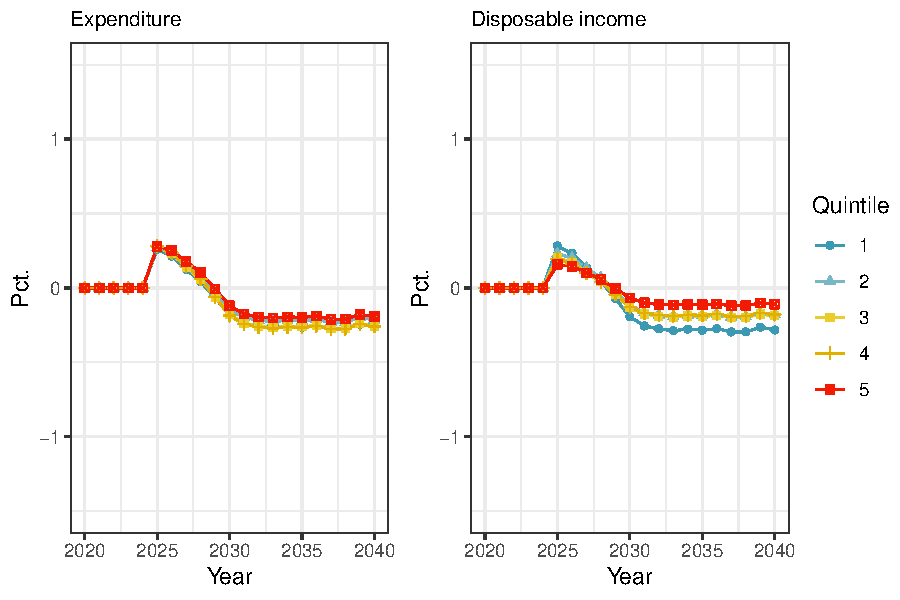
\includegraphics[width=.9\textwidth]{Figures/EV_P_tax1_hous.pdf}
\captionsetup{singlelinecheck=off,size=scriptsize}
\setlength{\captionmargin}{10pt}
\caption*{
\textbf{Note:} The price of housing is forced constant\\
\textbf{Source:} Own calculations based on the GreenREFORM model}
\end{figure}


\subsection{Distributional impact of income effects}
\subsubsection{Growth adjustment}

The price and wage changes after the tax are used to project consumption in our partial demand model in a scenario where income and consumption grows with the average growth rate, and a scenario where income and consumption grows with a differentiated growth rate across quintiles, as described in section \ref{sec:inc_growth}. 

An important assumption is the constant savings rate. This implies, that if income falls with a percent rate, total expenditure and total savings will fall with the same percent rate. Thus, the change in wage rate will equal the change in both disposable income \textit{and} total expenditure. In this analysis we do not focus on the effect on savings.


 To incorporate the change in the wage rate, we let income and expenditure grow with the average or differentiated growth rate $g_i$ (estimated in section \ref{sec:inc_growth}) for the period and the growth rate of the wage rate, calculated as: $g_{w,t} = \frac{w_t}{w_{t-1}}-1$. Thus, the projections of total expenditure, $\mu$, and disposable income, which we denote $M$, are:
 \begin{align}
    \mu_{i,t} = \mu_{i,t-1}(1+g_i+g_{w,t})
\end{align}
 \begin{align}
    M_{i,t} = M_{i,t-1}(1+g_i+g_{w,t})
\end{align}
where \textit{i} equals quintiles and \textit{t} goes from 2019 to 2040. An important assumption is underlying the above approach, namely that the "lost" income is distributed equally across quintiles. It is difficult to say how drops in the wage rate will be distributed across the income distribution, without explicitly modeling heterogeneous households with different productiveness. However, lower income groups might bear a larger risk of losing their jobs when total demand is reduced, a concern expressed by \cite{sune2020}. Further, a carbon tax might increase unemployment mostly for the less-educated, as shown in a Canadian study by \cite{YIP2018136}. More people from these groups receiving public transfers will make the tax more regressive than considered under the current assumptions. 

\subsubsection{Results with average growth rate}
In this section we want to analyze the income effects of a carbon tax, based on the three different tax scenarios as outlined in the previous section \ref{sec:tax_pd}. The results are presented as the income effect on welfare, EV$_I$, relative to total expenditure and disposable income. As seen, the income effect on consumption is neutral as share of total expenditure for all three scenarios. It is easy to resonate that this outcome will be neutral, since the total expenditure for each quintile grows with the same linear growth rate $g+g_w$. 
The income effect is negative and substantial compared to the price effect. This counts for all tax scenarios. The effect is largest for the third tax scenario, where rent on land is kept constant.

As the disposable income is distributed more unequal across quintiles than the total expenditure, the EV$_I$ is still regressive as share of disposable income. This is certainly because this analysis is a consumption analysis. The EV$_I$ measures the lost consumption due to an income change, but does not at all considers savings, since we do not have savings incorporated in our utility function. The effect on savings will be progressive. Thus the richer quintiles will give up more savings as share of their disposable income than the poorer quintiles.

\begin{figure}[H]
\centering
\caption{EV$_I$ relative to total expenditure and disposable income from a uniform 1500 CO2e tax}
\label{tax1_EV}
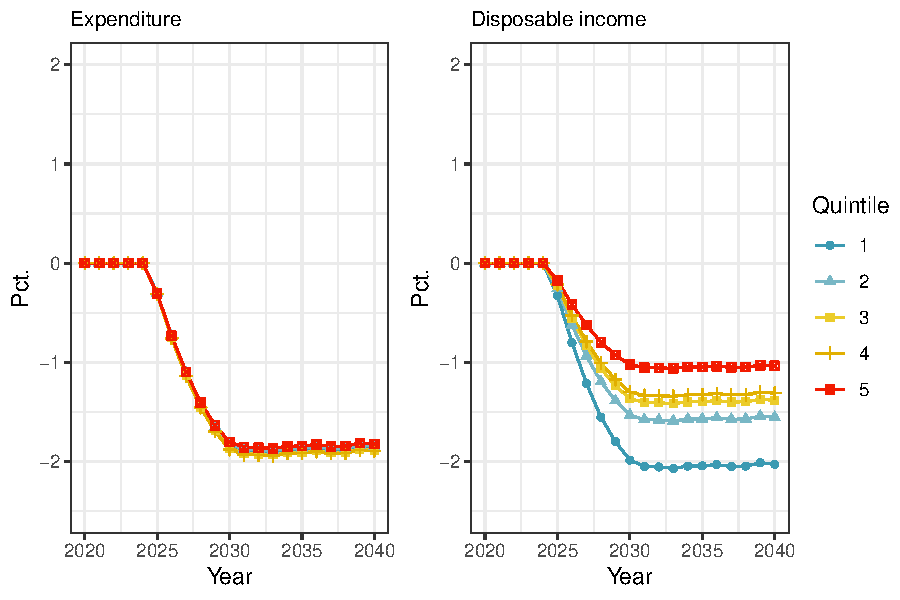
\includegraphics[width=.9\textwidth]{Figures/EV_tax1.pdf}
\captionsetup{singlelinecheck=off,size=scriptsize}
\setlength{\captionmargin}{10pt}
\caption*{
\textbf{Note:} Projections grow with the average growth rate\\
\textbf{Source:} Own calculations based on the GreenREFORM model}
\end{figure}

\begin{figure}[H]
\centering
\caption{EV$_I$ relative to total expenditure and disposable income from a 1250 CO2e tax on top of energy prices}
\label{tax2_EV}
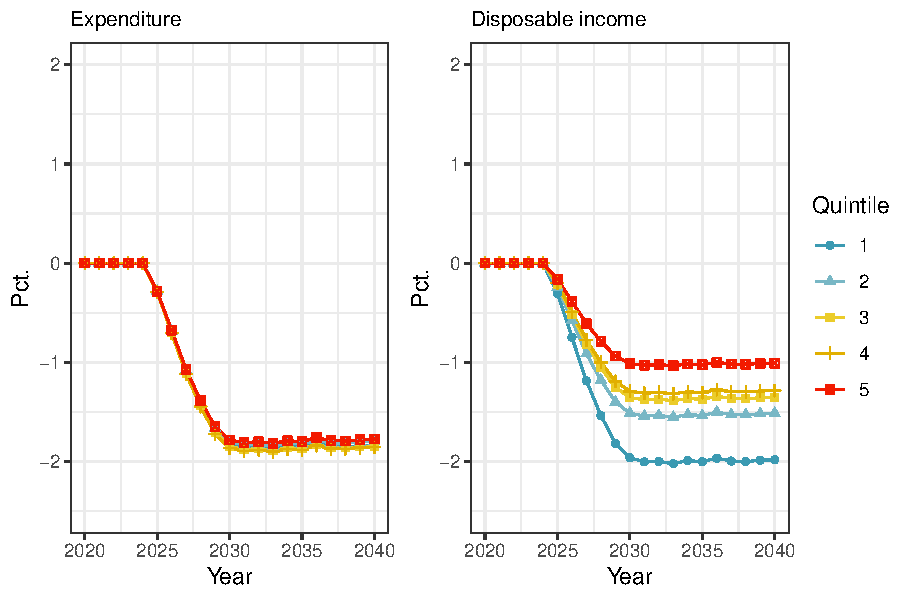
\includegraphics[width=.9\textwidth]{Figures/EV_tax2.pdf}
\captionsetup{singlelinecheck=off,size=scriptsize}
\setlength{\captionmargin}{10pt}
\caption*{
\textbf{Note:} Projections grow with the average growth rate\\
\textbf{Source:} Own calculations based on the GreenREFORM model}
\end{figure}

\begin{figure}[H]
\centering
\caption{EV$_I$ relative to total expenditure and disposable income from a uniform 1500 CO2e tax w. exogenous rent on land}
\label{tax3_EV}
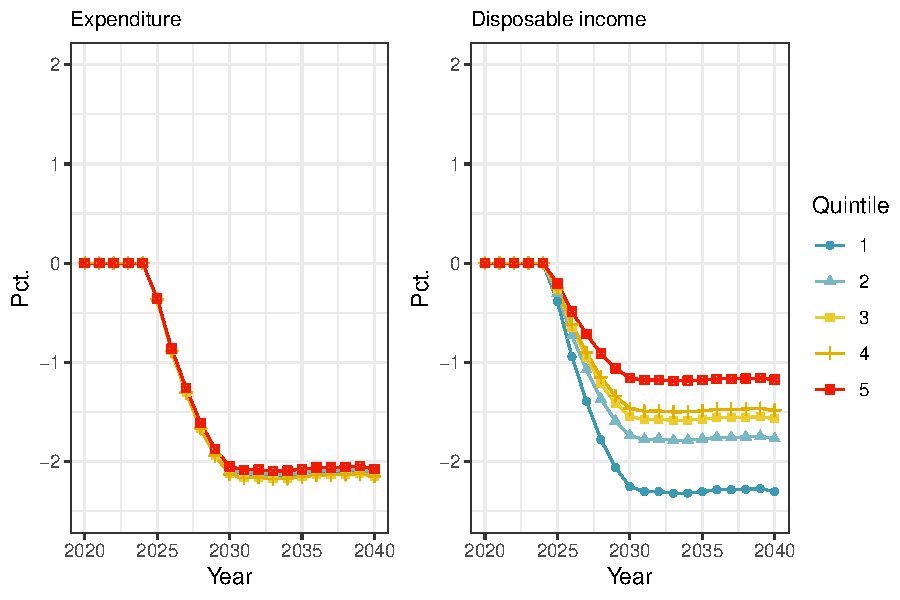
\includegraphics[width=.9\textwidth]{Figures/EV_tax3.pdf}
\captionsetup{singlelinecheck=off,size=scriptsize}
\setlength{\captionmargin}{10pt}
\caption*{
\textbf{Note:} Projections grow with the average growth rate\\
\textbf{Source:} Own calculations based on the GreenREFORM model}
\end{figure}

\subsubsection{Results with differentiated growth rates}
In this section we compare the results considering average growth with the results considering differentiated growth, and we print the absolute consumption losses for the different quintiles in DKK.

The table below shows the absolute income loss in DKK measured as the $EV_I$ in 2027 and 2035 for scenarios with average and differentiated growth rates. Quintile 1 loses between 4768 DKK and 5595 DKK of yearly income in 2035 and quintile 5 loses between 12761 DKK and 13587 DKK of yearly income in 2035. While the income loss for quintile 1 and 2 is smaller with differentiated growth than with average growth, since their growth rates are smaller than the average growth rate when differentiated. The opposite is the case for quintile 3, 4 and 5. This can also be interpreted as the higher quintiles compromising more future growth than the lower quintiles, which makes the absolute income effect less regressive than in the case of average growth rates.

\begin{table}[hhh]
\title{The income loss ($EV_I$) in DKK after a uniform CO2e tax of 1500 DKK}\label{tabel_EV_abs}
\centering
\begin{tabular}{@{}lllll@{}}
\toprule
 & \multicolumn{2}{l}{Average growth} & \multicolumn{2}{l}{Differentiated growth} \\ \midrule
\textbf{Year} & \textbf{2027} & \textbf{2035} & \textbf{2027} & \textbf{2035} \\
Quintile 1 & -4509.63 & -5595.46 & -3390.7 & -4767.66 \\
Quintile 2 & -5493.09 & -6815.71 & -4246.57 & -6139.41 \\
Quintile 3 & -7250.03 & -8995.69 & -5909.57 & -9008.21 \\
Quintile 4 & -7995.94 & -9921.2 & -6615.75 & -10236.6 \\
Quintile 5 & -10285 & -12761.4 & -8644.37 & -13587.2 \\ \bottomrule
\end{tabular}
\caption*{
\textbf{Source:} Own calculations}
\end{table}

However, when regressivity is measured as share of total expenditure, the income effect in the scenario of differentiated growth rates is actually more regressive, since the total expenditure of the higher quintiles grow more than the lower quintiles'. However the effect is so small compared to total expenditure that it's difficult to see in the plot, see figure \ref{EV_diff}.

\begin{figure}[H]
\centering
\caption{EV relative to total expenditure and disposable income from a uniform 1500 CO2e tax where growth rates are differentiated}
\label{EV_diff}
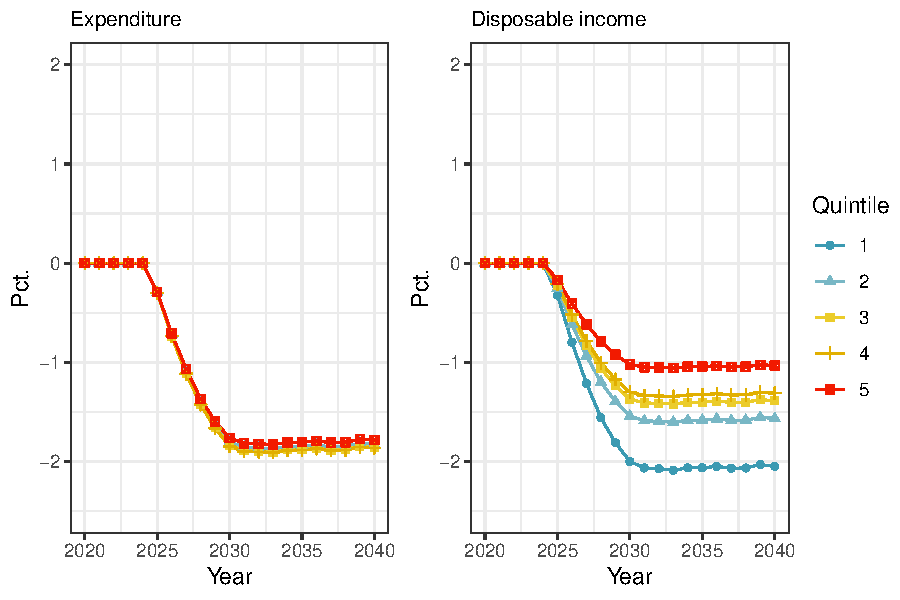
\includegraphics[width=.9\textwidth]{Figures/EV_plot_diff.pdf}
\captionsetup{singlelinecheck=off,size=scriptsize}
\setlength{\captionmargin}{10pt}
\caption*{
\textbf{Note:} Projections with differentiated growth\\
\textbf{Source:} Own calculations}
\end{figure}


